\chapter{Conceptual Overview} \label{sec:conceptual}

GEX is designed to be modular and easy to extend. The user-facing functionality is composed of independent software modules, called \textit{functional blocks} or \textit{units}, which can be configured by the user to fit their application needs. Units implement low-level logic to work with hardware peripherals of the microcontroller, and expose this functionality to the client application, running on the \gls{PC}, through a communication interface. A diagram showing the entire stack, from the user application down to hardware peripherals, is shown in \cref{fig:conceptual}.

\begin{figure}[h]
	\centering
	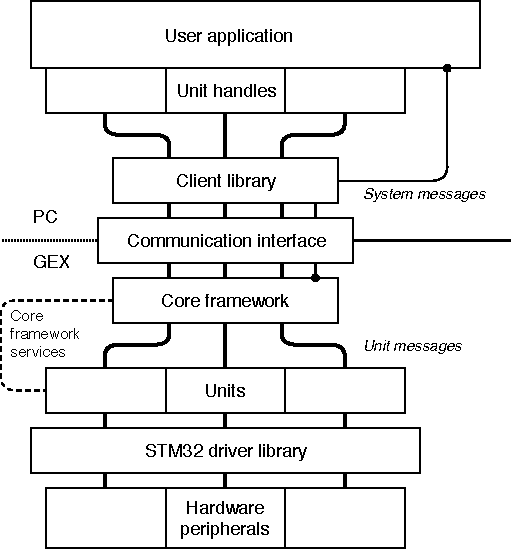
\includegraphics[scale=1]{img/conceptual.pdf}
	\caption[GEX conceptual overview]{\label{fig:conceptual}The ``GEX stack'', from a user application down to hardware}
\end{figure}

When we work with GEX, it is through units. The platform without units would be just an empty shell, the bare core framework; this underlying system will be described in \cref{sec:coreframework}. We will explore the individual units in \cref{sec:units_overview}, after going through the hardware realizations in \cref{sec:hwreal} and covering the communication protocol in \cref{sec:tinyframe}. 

\section{Physical User Interface}

The firmware can be flashed to a STM32 development board, or a custom \gls{PCB}. The particulars of those form factors will be discussed in \cref{sec:hwreal}.

\begin{figure}[h]
	\centering
	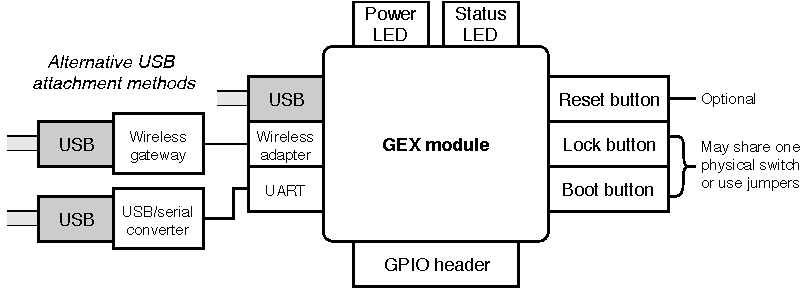
\includegraphics[scale=.95] {img/users-view.pdf}
	\caption{\label{fig:users_view_of_gex}Physical user interface of a GEX module}
\end{figure}

\noindent
All GEX hardware platforms have some common characteristics (\cref{fig:users_view_of_gex}):

\begin{itemize}	
	\item \textbf{Power \gls{LED}} -- a simple indication that the board is powered on
	\item \textbf{Status \gls{LED}} -- periodic flashing every 3\,s indicates correct operation, continuous light a software error\footnote{The microcontroller will then automatically restart within a few seconds due to a watchdog timeout.}; other light patterns may be shown as feedback to user actions or received commands
	\item \textbf{Reset button} -- resets the \gls{MCU}; this is particularly useful during firmware development as an alternative to re-connecting the \gls{USB} cable
	\item \textbf{Lock button} -- enables or disables access to configuration files through the virtual mass storage device
	\item \textbf{Boot button} -- when held during restart (that is, while the reset button is released), the \gls{DFU} mode~\cite{usbif-dfu} is activated and a new firmware image can be flashed over the \gls{USB} connection using \mono{dfu-util}~\cite{dfu-util} or other firmware update application
	\item \textbf{\gls{GPIO} header} -- a pin header exposing the \gls{MCU}'s \gls{GPIO} pins to be connected to external circuitry
	\item \textbf{Communication interface} -- a connection to the host \gls{PC}; multiple options may be available to choose from, a direct \gls{USB} connection being the primary and always available option
\end{itemize}

\section{GEX-PC Connection}

\Cref{fig:users_view_of_gex} shows three ways to connect the module to a \gls{PC}. Each communication interface has its advantages and drawbacks, and is suitable for different use-cases.

\begin{itemize}
	\item \textbf{Direct \gls{USB} connection}
		
		This is the primary and most straightforward connection method. We use the \gls{CDCACM} and \gls{MSC} \gls{USB} classes to have the module appear as a virtual COM port and a mass storage device, as described in \cref{sec:usb_classes}. This method is the fastest of the three and works out-of-the-box on Linux and MacOS. On MS Windows it may require the right software driver to be installed and assigned manually\footnote{The STM32 virtual COM port driver~\cite{stm-vcom} has been tested to work with GEX on MS Windows version 7 and 8, though it must be manually assigned to the device in the Device Manager. MS Windows 10 and later should support \gls{CDCACM} as a virtual COM port natively.}.
	
	\item \textbf{Hardware \gls{UART}}
	
		The hardware UART used as a communication interface is mapped to pins PA2 and PA3 to be compatible with the built-in \gls{USB}/\gls{UART} converter on STM32 Nucleo development boards. This interface is functionally identical to the \gls{CDCACM} connection, but the physical \gls{UART} is necessarily slower and does not implement flow control.
		
	\item \textbf{Wireless connection}
	
		A wireless connection is implemented using a radio module on the GEX board. To use it we need a counterpart, the \textit{wireless gateway}, which connects to the \gls{PC} via \gls{USB} and acts as a \gls{CDCACM} device.
	
\end{itemize}

The \gls{USB} connection is always enabled first on start-up. GEX waits its for enumeration by the host \gls{PC}. When not enumerated in a few seconds, it concludes that the interface is not active and tries other enabled options. The wireless module, connected through \gls{SPI}, can be detected by reading one of its registers that should have a known value. A \gls{UART} interface cannot be tested so reliably, thus it is always considered active\footnote{A detection of the UART connection would be possible by measuring the Rx pin voltage, which should idle at a high level (here 3.3\,V). This was not implemented in the initial firmware version.}.

\section{Controlling GEX}

GEX is a platform providing access to low-level hardware to high-level applications. However, this ``high level'' is relative. As was shown in \cref{fig:conceptual}, the ``GEX stack'' ends with a \textit{client library}, a software library used by the \textit{user application}.

The communication protocol (one level lower in the diagram), which will be explained in \cref{sec:tinyframe}, may be implemented as part of the client library in any programming language and on any platform; in theory, it is even possible to control GEX from another microcontroller. The client library implements, besides the protocol itself, other higher-level logic, and gives the user access to individual units using an abstraction called \textit{unit handles}.

Any logic above the client library is in the hands of the user, which means that, to use GEX, they have to program a user application. Proof-of-concept client libraries in languages C and Python are provided for this purpose, and will be explained in \cref{sec:clientsw}.

\section{Device Configuration}

The core framework and each of the units have a number of adjustable options determining their behavior. Those settings are internally stored in a binary form, but to make their adjustment comfortable for the user, they are mapped to text configuration files in the INI format.

\subsection{INI File Format}

INI files are, in our implementation, simple text files containing three basic syntax elements: comments, sections, and key-value entries. Sections group the key-value pairs into logical blocks, e.g., the configuration of individual units.

\begin{itemize}	
	\item \textbf{Comments} start with the hash symbol (\mono{\#}) and end at the end of line
	\item \textbf{Sections} are textual labels enclosed in square brackets (\mono{[UNITS]})
	\item \textbf{Key-value entries} are composed of a label, the equals sign, and its value; values may be text strings, decimal or hexadecimal numbers, lists of numbers separated by commas, or any other format appropriate for the particular key
\end{itemize}

\noindent
An example of the INI syntax is shown below.

\begin{inicode}
# comment
[section]
a = 123
b = 0xFF
port = A
pins = 1,2,3
\end{inicode}
	
\subsection{Configuration Files Structure}

The configuration is split into two files: \mono{UNITS.INI} and \mono{SYSTEM.INI}. The system configuration file has a simple structure and does not need much explanation beyond the comments already included in it; an example of its content is captured in \cref{lst:systemini}. The other file, as its name suggests, serves to configure GEX units.

\begin{listing}
	\begin{inicode}
		## SYSTEM.INI
		
		[SYSTEM]
		# Data link accessible as virtual comport (Y, N)
		expose-vcom=Y
		# Show comments in INI files (Y, N)
		ini-comments=Y
		# Enable debug UART-Tx on PA9 (Y, N)
		debug-uart=Y
		
		# Output core clock on PA8 (Y, N)
		mco-enable=N
		# Output clock prediv (1,2,...,128)
		mco-prediv=128
		
		# --- Allowed fallback communication ports ---
		
		# UART Tx:PA2, Rx:PA3
		com-uart=N
		com-uart-baud=115200
		
		# nRF24L01+ radio
		com-nrf=N
		# Radio channel (0-125)
		nrf-channel=76
		# Network prefix (hex, 4 bytes)
		nrf-network=12:00:09:4C
		# Node address (1-255)
		nrf-address=1
	\end{inicode}
	\caption{\label{lst:systemini}The \mono{SYSTEM.INI} configuration file}
\end{listing}

\begin{listing}
	\begin{inicode}
		## UNITS.INI
		
		[UNITS]
		# Create units by adding their names next to a type (e.g. DO=A,B),
		# remove the same way. Reload to update the unit sections below.
		
		# Digital output
		DO=led
		# Digital input with triggers
		DI=btn1,btn2
		# Neopixel RGB LED strip
		NPX=
		# I2C master
		I2C=i2c
		#...
		
		[I2C:i2c@1]
		# Peripheral number (I2Cx)
		#...
	\end{inicode}
	\caption{\label{lst:unitsini}Part of the \mono{UNITS.INI} configuration file}
\end{listing}

The units file, illustrated in \cref{lst:unitsini}, is more complex, and \textit{interactive}. The top part, a \mono{[UNITS]} section, lists all available unit types. A unit is created by writing its name (an arbitrary label composed of letters, numbers, and underscore) next to the desired type. Each unit is then configured in a separate section lower in the file; however, how does one know what keys are needed for which unit? This problem is solved by \textit{interactivity} of the file.

After adding a unit name next to its type, we save the file. The disk temporarily disappears from the device list as the file's content updates. When we reopen the file, a section for the new unit will be appended for us to configure as necessary. To delete a unit, it is sufficient to remove its name from the list at the top and let the file regenerate the same way; the unit's section will disappear.

It is not uncommon that the entered (or default) configuration is invalid and the unit cannot be enabled. The error is reported by inserting a comment into the INI file, at the top of the section of the failing unit. This error message disappears when the problem is corrected.

Once we are satisfied with the configuration, it may be stored to the module's permanent memory. This is done by pushing the Lock button again, which also deactivates the virtual storage device.

It may be interesting to know that the configuration files can also be read and modified through the communication interface. A simple configuration editor (\cref{fig:gexync}) was developed to demonstrate this feature. Besides applications like this, we can use the programmatic configuration access to change GEX settings automatically by the client application. The changes may be persisted by a command, but that is not required, which lets us use them temporarily without modifying the stored configuration.

\begin{figure}
	\centering
	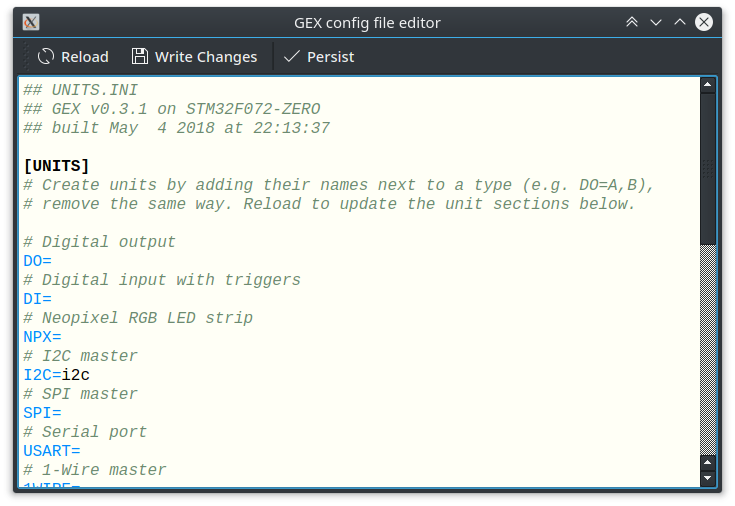
\includegraphics[width=.8\textwidth] {img/gexync.png}
	\caption[Configuration file editor GUI]{\label{fig:gexync}Configuration file editor GUI built using the GEX client library and PyQt4}
\end{figure}



















